\documentclass[10pt,a4paper,twocolumn]{article}

\usepackage[utf8]{inputenc}
\usepackage[T1]{fontenc}
\usepackage[english]{babel}
\usepackage{lmodern}
\usepackage{microtype}
\usepackage{csquotes}
\usepackage{hyperref}
\usepackage{geometry}
\usepackage{graphicx}
\usepackage{booktabs}
\usepackage{enumitem}
\usepackage[numbers,sort&compress]{natbib}

\geometry{margin=2.5cm}
\setlist{nosep}

\title{PORTUWiC-BR: A Word-in-Context Benchmark for Brazilian Portuguese}
\author{XXX}

\begin{document}

\maketitle

\begin{abstract}
\end{abstract}

\section{Introduction}

\section{Background}
\label{sec:background}

This section reviews the foundations required for building PORTUWiC-BR. It first introduces the Word-in-Context task and its relation to Word Sense Disambiguation, then discusses how WiC-style datasets have been constructed in previous work.

\subsection{The Word-in-Context Task}
\label{subsec:wic-task}

The Word-in-Context (WiC) task was proposed as a way to evaluate context-sensitive meaning representations without requiring a model to output a sense identifier from a fixed lexical inventory. Instead of framing lexical disambiguation as a classification problem over predefined senses, WiC presents two occurrences of the same target word in two contexts and asks whether the two uses correspond to the same meaning \citep{pilehvar2019wic}. This formulation turns a traditional Word Sense Disambiguation (WSD) problem into a binary task, making it suitable for evaluating contextualized models and systems that do not explicitly operate over dictionary senses.

In a standard WiC instance, the input contains a target word, two sentences in which that target occurs, and a binary label indicating whether the two occurrences express the same sense. This format differs from classical WSD because the model is not asked to choose among all possible dictionary senses of a word. Instead, it must compare two contextualized uses directly. This makes the task useful for evaluating whether a model captures the dynamic nature of lexical meaning, since the same form may preserve its meaning across contexts or shift to a different sense depending on surrounding words, syntax, genre, or pragmatic setting.

The WiC formulation has also motivated multilingual and cross-lingual variants. XL-WiC extends WiC to twelve additional languages and supports evaluation of cross-lingual transfer \citep{rahnama2020xlwic}. MCL-WiC, introduced at SemEval-2021, formulates both multilingual and cross-lingual Word-in-Context disambiguation, asking systems to compare word meanings either within the same language or across different languages \citep{martelli2021mclwic}. These datasets reinforce the view that WiC evaluation should measure the ability to discriminate senses in context without requiring the system's output to be structured by a fixed sense inventory.

For a Brazilian Portuguese benchmark, this task formulation is especially relevant because it allows the evaluation of contextual understanding in polysemous, idiomatic, colloquial, and regional uses without forcing the model to select a dictionary entry as its final answer. For example, the word \enquote{arretado} may express a positive evaluation in one context and irritation in another; a WiC benchmark can represent this contrast directly as a pairwise semantic decision.

In the Portuguese context, Gon{\c{c}}alves \citep{goncalves2024filling} proposes resources to fill gaps in European Portuguese benchmarks, including WiC. The work highlights that directly translating English datasets may compromise the task, since the target word or the original ambiguity may disappear in translation. To build a European Portuguese WiC dataset, the author combines data from a multilingual study on homonymy and synonymy, examples from the \textit{Dicionario Gramatical de Verbos do Portugues}, and a data augmentation step using ChatGPT. This methodological design is relevant to Brazilian Portuguese because it points to an alternative to direct translation in which instances are built from language-specific resources and, when necessary, complemented through controlled generation and human review.

\subsection{Construction Strategies in WiC-style Datasets}
\label{subsec:methods-creation}

Existing WiC-style benchmarks differ not only in the languages they cover, but also in how candidate sentence pairs are obtained and validated. The most common strategy is to exploit lexical resources that already organize words into senses. This is the case for the original English WiC dataset, which uses examples from WordNet, VerbNet and Wiktionary \citep{pilehvar2019wic}, and for XL-WiC, which extends this approach with multilingual WordNets and Wiktionary entries \citep{rahnama2020xlwic}. This strategy is attractive because sense inventories provide an initial semantic structure in which examples attached to the same sense can be paired as positive instances, whereas examples attached to different senses can be paired as negative instances. Its main limitation is coverage, since many languages, domains, and regional varieties lack sense inventories with enough examples.

Another strategy is to select naturally occurring corpus examples and annotate them manually. MCL-WiC follows this direction by using BabelNet to select ambiguous lexemes, extracting sentence pairs from the United Nations Parallel Corpus and Wikipedia, and relying on annotators with language proficiency to assign the same-sense or different-sense labels \citep{martelli2021mclwic}. This approach is more expensive than automatic pairing from dictionary examples, but it offers greater control over domains, genres, parts of speech, and cross-lingual settings. It also shows that lexicographic resources can support target-word selection without fully determining the final labels.

A third route uses hyperlinks or entity/concept links as a form of distant supervision. AM2iCo builds multilingual and cross-lingual meaning-in-context datasets from Wikipedia, using the context of hyperlinked words and Wikipedia cross-lingual links to infer whether two occurrences point to the same concept \citep{liu2021am2ico}. Positive examples can be formed when occurrences link to the same page, while negative examples can be formed when the same surface form links to different pages. The authors also add filtering heuristics and adversarial examples, showing that dataset construction can explicitly target cases that are difficult for models rather than only cases that are easy to collect.

A related but slightly different formulation is Target Sense Verification (TSV), where a model receives one context and one candidate sense, represented for instance by a definition or hypernym, and decides whether the context expresses that sense. WiC-TSV is built partly from WiC and partly from domain-specific resources, including thesauri, MeSH, Wikipedia, Wikilinks, search-engine contexts, and manual expert decisions \citep{breit2021wictsv}. Although TSV is not identical to WiC, it is relevant for dataset design because it shows how definitions, hypernyms, domain resources, and manually gathered contexts can be combined when a full sense inventory is incomplete or unavailable.

More recently, LLMs have become a possible tool for data annotation and synthetic data generation, but the literature emphasizes that generated or model-labeled data requires curation, verification, and human evaluation, especially for tasks involving fine-grained semantic judgments \citep{ding2024llmannotation,long2024syntheticdata}.

\section{Methodology}
\label{sec:methodology}

The construction of PORTUWiC-BR follows a hybrid methodology that combines lexical resources, LLM-assisted generation, automatic filtering, and linguistic validation. The pipeline is designed to produce candidate WiC instances for Brazilian Portuguese while preserving explicit information about the target word, its contexts, the source of each instance, and its validation status. Figure~\ref{fig:methodology} summarizes the main stages of the proposed process.

\begin{figure*}[t]
    \centering
    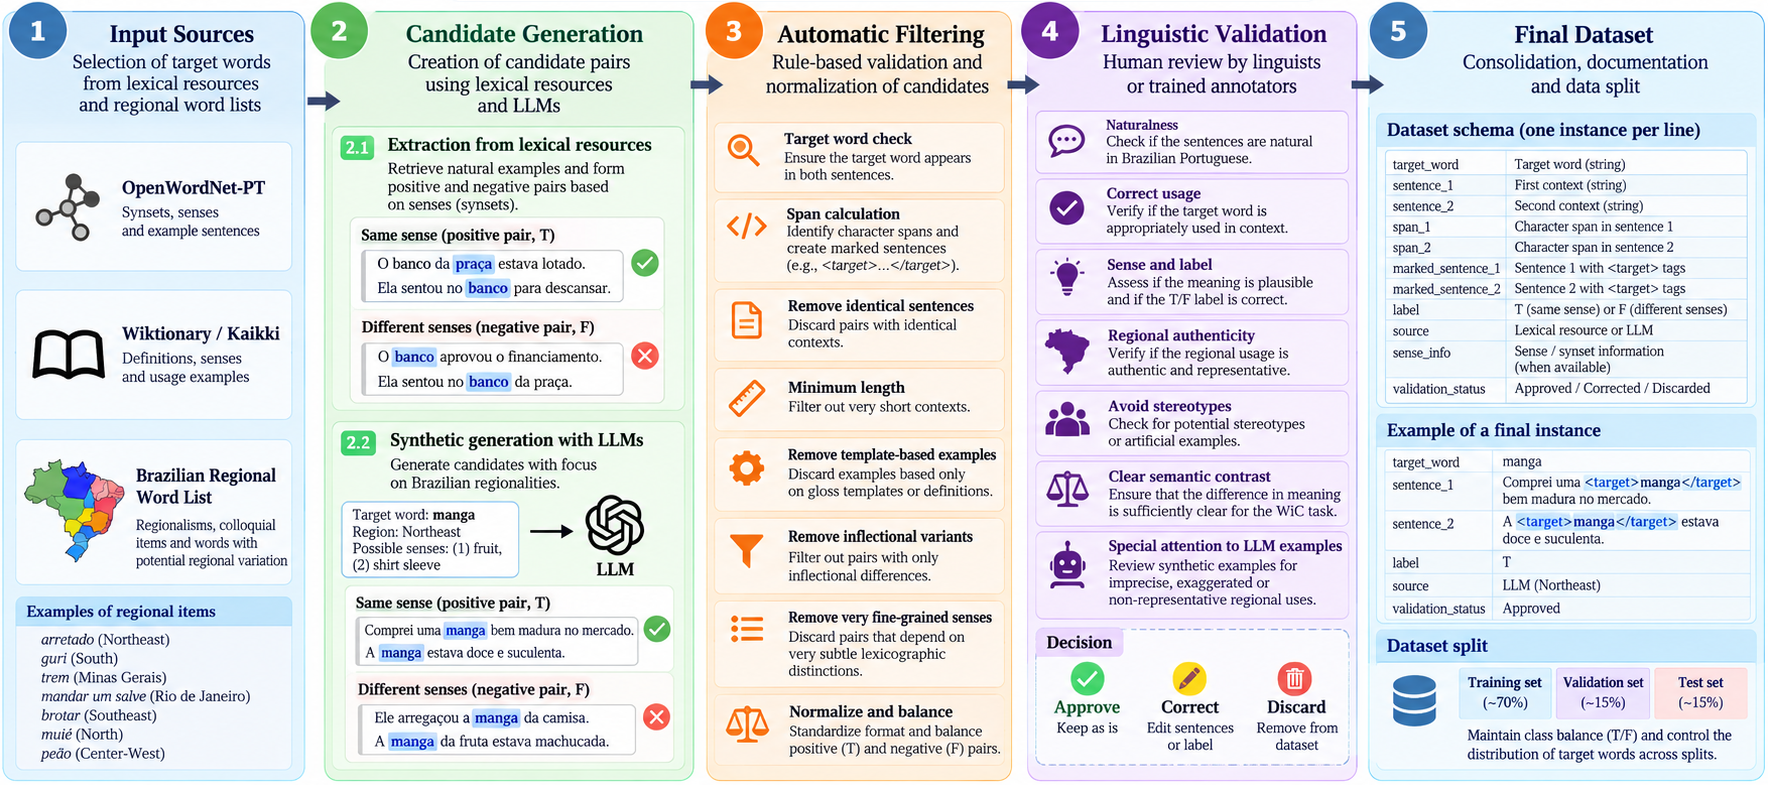
\includegraphics[width=\textwidth]{images/methodology.png}
    \caption{Overview of the proposed methodology for constructing PORTUWiC-BR.}
    \label{fig:methodology}
\end{figure*}

\subsection{Input Sources}
\label{subsec:input-sources}

The first stage consists of selecting candidate target words and collecting initial evidence about their possible meanings. We consider three main sources. The first is OpenWordNet-PT, which provides Portuguese lemmas associated with synsets and lexical-semantic information. The second is Wiktionary, accessed through the Kaikki/Wiktextract dump, which provides dictionary entries, definitions, part-of-speech information, and usage examples when available. The third is a manually curated seed list of Brazilian regional and colloquial words, including items associated with the Northeast, North, South, Minas Gerais, Rio de Janeiro, São Paulo, Central Brazil, and other regional varieties.

The regional list is not intended to define the final coverage of the benchmark. Instead, it serves as a controlled starting point for identifying words whose meanings may vary across regions or contexts. Examples include terms whose senses may shift between literal, colloquial, evaluative, and regionally marked uses. This design allows the dataset to include general polysemy as well as semantic variation that is especially relevant to Brazilian Portuguese.

\subsection{Candidate Generation}
\label{subsec:candidate-generation}

The second stage creates candidate sentence pairs from the input sources. It is divided into two complementary routes. The first route extracts candidate pairs from lexical resources, while the second route uses LLMs to generate synthetic examples focused on Brazilian regional variation.

\subsubsection{Extraction from Lexical Resources}
\label{subsubsec:lexical-extraction}

Lexical candidates are generated from OpenWordNet-PT and Kaikki/Wiktionary. In this stage, the pipeline searches for cases in which the same Portuguese target word appears in examples associated with one or more senses. Positive pairs are created when two examples are linked to the same sense or synset. Negative pairs are created when the same target word appears in examples associated with different senses or synsets.

The generation procedure only keeps examples in which the target word appears explicitly in both sentences. This constraint is important because the WiC task requires the model to compare two occurrences of the same lexical item. The pipeline therefore computes the character span of the target word in each sentence and stores both the raw sentence and a marked version of the sentence with the target occurrence delimited by \texttt{<target>} and \texttt{</target>}. Candidate pairs based only on gloss templates are excluded by default, since template-based contexts may introduce artificial regularities and make the task less representative of natural language use.

\subsubsection{Synthetic Generation with LLMs}
\label{subsubsec:llm-generation}

The lexical resources used in the first route do not fully cover regional and colloquial meanings in Brazilian Portuguese. To address this limitation, a second route uses LLM-assisted generation to propose candidate examples for regional vocabulary. The generation seed consists of 200 target words manually organized with a regional hint and a short semantic note. The list includes items such as \textit{arretado}, \textit{azuado}, \textit{brabo}, \textit{dindin}, \textit{mangarataia}, and \textit{chimarrão}. Each model call produces one candidate dataset row containing two Brazilian Portuguese sentences, the intended label, short sense descriptions, and a brief rationale.

For reproducibility, the current generation script uses the OpenAI Responses API with model \texttt{gpt-5-mini}, temperature \texttt{0.7}, and structured JSON output. The generation order is controlled with random seed \texttt{13}. The full generation plan contains 200 calls, divided into 100 positive candidates and 100 negative candidates. The output schema requires the target word, label, two sentences, two sense descriptions, regional information, and a rationale. The target word is then checked locally, and examples are kept only when the same spelling appears in both sentences.

The LLM generation process is controlled by explicit constraints. The target word must appear exactly once in each sentence and must keep the same spelling in both contexts. For positive examples, the two occurrences must express the same meaning. For negative examples, the two occurrences must express clearly different meanings. The prompt also instructs the model to avoid dictionary definitions, metalinguistic explanations, and repeated templates. These restrictions are intended to make the generated examples closer to natural usage and to reduce superficial cues that could simplify the task.

Some generated candidates illustrate the intended behavior of this route. For a negative pair with \textit{tangerina}, the model produced \enquote{No fim da tarde comi uma tangerina suculenta enquanto esperava o ônibus} and \enquote{Decidimos pintar a parede da sala de tangerina para combinar com as almofadas}, contrasting a fruit sense with a color sense. For \textit{dindin}, another negative pair contrasts a frozen dessert in \enquote{as crianças correram até o carrinho para comprar um dindin de coco} with a money sense in \enquote{Sem um dindin no bolso, ele teve que adiar a viagem}. For a positive pair with \textit{brabo}, both contexts use the word with the sense of being dangerous or difficult to handle, as in \enquote{o tempo ficou brabo} and \enquote{o touro estava brabo}. These examples remain candidates and are not considered final annotations before linguistic review.

LLM-generated examples are treated only as candidates. They are marked as synthetic and assigned a pending validation status. This distinction is important because a generated sentence may sound plausible while still containing an inaccurate regional use, an exaggerated stereotype, or a semantic contrast that is not stable for Brazilian Portuguese speakers. For this reason, LLM generation is used as a coverage-expansion mechanism rather than as an authoritative annotation source.

\subsection{Automatic Filtering}
\label{subsec:filtering-normalization}

After candidate generation, all examples pass through automatic filtering and schema normalization. The filtering step removes rows in which the target word is absent from one of the two sentences, rows with identical sentences, very short contexts, and entries that correspond only to inflectional forms rather than lexical senses. The pipeline also removes or deprioritizes cases in which the semantic distinction appears to be too fine-grained for a reliable WiC decision.

All accepted candidates are converted to a shared schema. Each row stores the target word, the two contexts, the target spans, the marked sentences, the binary label, sense descriptions when available, the generation source, and the validation status. This shared representation makes it possible to combine candidates from lexical resources and from LLM generation while preserving information about provenance.

\subsection{Linguistic Validation}
\label{subsec:linguistic-validation}

The central quality-control stage is linguistic validation. A linguist or trained annotators review the automatically generated candidates and decide whether each instance should be accepted, corrected, or discarded. The review focuses on several criteria. First, the annotator verifies whether both sentences are natural in Brazilian Portuguese. Second, the annotator checks whether the target word is correctly identified and whether its occurrence is the one that should be compared. Third, the annotator evaluates whether the assigned label is semantically appropriate.

For positive pairs, the annotator checks whether the two occurrences of the target word express the same meaning in context. For negative pairs, the annotator verifies whether the contrast between senses is clear enough for a WiC benchmark. Cases that depend on excessively subtle dictionary distinctions are removed or revised, since such distinctions may reduce annotation reliability. This step is especially important for resources based on WordNet-like inventories, where some sense divisions may be finer than what is useful for the binary WiC formulation.

The validation of regional and LLM-generated examples requires additional care. The annotator assesses whether the regional use is authentic, whether it is compatible with the indicated variety, and whether the example avoids caricature or stereotyped language. If a regional term has multiple uses, the annotator may refine the sense description or replace a generated sentence with a more natural alternative. The final label is therefore determined by linguistic judgment rather than by the lexical resource or by the LLM output alone.

\subsection{Final Dataset}
\label{subsec:dataset-consolidation}

After validation, accepted instances are consolidated into the final dataset. The dataset is balanced between positive and negative labels whenever possible. The split into training, development, and test sets is created after deduplication and normalization. The split should preserve label balance and avoid excessive repetition of the same sentences. Depending on the evaluation goal, it may also control the distribution of target words across partitions in order to measure lexical generalization.

The final dataset documentation records the source of each instance, the validation status, and any relevant information about regional use. This documentation is necessary for later error analysis and for comparing the behavior of models on examples derived from lexical resources, examples generated with LLM assistance, and examples involving Brazilian regional variation.

\section{Experiments}

\section{Results and Discussion}

\section{Conclusion}

\bibliographystyle{plainnat}
\bibliography{references}

\end{document}
